%%%%%%%%%%%%%%%%%%%%%%%%%%%%%%%%%%%%%%%%%
% Beamer Presentation
% LaTeX Template
% Version 1.0 (10/11/12)
%
% This template has been downloaded from:
% http://www.LaTeXTemplates.com
%
% License:
% CC BY-NC-SA 3.0 (http://creativecommons.org/licenses/by-nc-sa/3.0/)
%
%%%%%%%%%%%%%%%%%%%%%%%%%%%%%%%%%%%%%%%%%

%----------------------------------------------------------------------------------------
%	PACKAGES AND THEMES
%----------------------------------------------------------------------------------------

\documentclass[UTF8,aspectratio=169,12pt]{ctexbeamer}

\usepackage{hyperref}
\hypersetup{
	colorlinks=true,
	linkcolor=red,
	anchorcolor=blue,
	citecolor=green
}

\mode<presentation> {
	
	% The Beamer class comes with a number of default slide themes
	% which change the colors and layouts of slides. Below this is a list
	% of all the themes, uncomment each in turn to see what they look like.
	
	%\usetheme{default}
	%\usetheme{AnnArbor}
	%\usetheme{Antibes}
	%\usetheme{Bergen}
	%\usetheme{Berkeley}
	%\usetheme{Berlin}
	%\usetheme{Boadilla}
	%\usetheme{CambridgeUS}
	%\usetheme{Copenhagen}
	%\usetheme{Darmstadt}
	%\usetheme{Dresden}
	%\usetheme{Frankfurt}
	%\usetheme{Goettingen}
	%\usetheme{Hannover}
	%\usetheme{Ilmenau}
	%\usetheme{JuanLesPins}
	%\usetheme{Luebeck}
	\usetheme{Madrid}
	%\usetheme{Malmoe}
	%\usetheme{Marburg}
	%\usetheme{Montpellier}
	%\usetheme{PaloAlto}
	%\usetheme{Pittsburgh}
	%\usetheme{Rochester}
	%\usetheme{Singapore}
	%\usetheme{Szeged}
	%\usetheme{Warsaw}
	
	% As well as themes, the Beamer class has a number of color themes
	% for any slide theme. Uncomment each of these in turn to see how it
	% changes the colors of your current slide theme.
	
	%\usecolortheme{albatross}
	%\usecolortheme{beaver}
	%\usecolortheme{beetle}
	%\usecolortheme{crane}
	%\usecolortheme{dolphin}
	%\usecolortheme{dove}
	%\usecolortheme{fly}
	%\usecolortheme{lily}
	%\usecolortheme{orchid}
	%\usecolortheme{rose}
	%\usecolortheme{seagull}
	%\usecolortheme{seahorse}
	%\usecolortheme{whale}
	%\usecolortheme{wolverine}
	
	%\setbeamertemplate{footline} % To remove the footer line in all slides uncomment this line
	%\setbeamertemplate{footline}[page number] % To replace the footer line in all slides with a simple slide count uncomment this line
	
	%\setbeamertemplate{navigation symbols}{} % To remove the navigation symbols from the bottom of all slides uncomment this line
}

\usepackage{graphicx} % Allows including images
\graphicspath{{./figs/}}
\usepackage{booktabs} % Allows the use of \toprule, \midrule and \bottomrule in tables
\usepackage{longtable}
\usepackage{xcolor}
\usepackage{minted}
\usepackage{listings}
\lstset{numbers=left, %设置行号位置
	numberstyle=\tiny, %设置行号大小
	keywordstyle=\color{blue}, %设置关键字颜色
	commentstyle=\color[cmyk]{1,0,1,0}, %设置注释颜色
	frame=single, %设置边框格式
	escapeinside=``, %逃逸字符(1左面的键),用于显示中文
	%breaklines, %自动折行
	extendedchars=false, %解决代码跨页时,章节标题,页眉等汉字不显示的问题
	xleftmargin=2em,xrightmargin=2em, aboveskip=1em, %设置边距
	tabsize=4, %设置tab空格数
	showspaces=false %不显示空格
}
% Fonts
% \usepackage{libertine}
% \setmonofont{Courier}
%\setCJKsansfont[ItalicFont=Noto Serif CJK SC Black, BoldFont=Noto Sans CJK SC Black]{Noto Sans CJK SC}


%----------------------------------------------------------------------------------------
%	TITLE PAGE
%----------------------------------------------------------------------------------------

\title[第1讲]{第1讲 :操作系统概述} % The short title appears at the bottom of every slide, the full title is only on the title page
\subtitle{第一节:课程概述\&教学安排}
\author{向勇、陈渝、李国良} % Your name
\institute[清华大学] % Your institution as it will appear on the bottom of every slide, may be shorthand to save space
{
清华大学计算机系 \\ % Your institution for the title page
\medskip
\textit{xyong,yuchen,liguoliang@tsinghua.edu.cn} % Your email address
}
\date{\today} % Date, can be changed to a custom date

\begin{document}

\begin{frame}
\titlepage % Print the title page as the first slide
\end{frame}

%\begin{frame}
%\frametitle{提纲} % Table of contents slide, comment this block out to remove it
%\tableofcontents % Throughout your presentation, if you choose to use \section{} and \subsection{} commands, these will automatically be printed on this slide as an overview of your presentation
%\end{frame}
%
%%----------------------------------------------------------------------------------------
%%	PRESENTATION SLIDES
%%----------------------------------------------------------------------------------------
%
%%------------------------------------------------
%\section{第二节:教学安排} % Sections can be created in order to organize your presentation into discrete blocks, all sections and subsections are automatically printed in the table of contents as an overview of the talk
%%------------------------------------------------
\begin{frame}
    \frametitle{提纲}
    \begin{itemize}
        \item 第一节 课程概述&教学安排
        \item 第二节 什么是操作系统
        \item 第三节 操作系统历史演变
        \item 第四节 操作系统结构
        \item 第五节 OS实验概述
    \end{itemize}
\end{frame}
%%------------------------------------------------
\begin{frame}
    \frametitle{课程信息}
    \begin{itemize}
        \item 主讲教师:
        \begin{itemize}
            \item 向勇
        \end{itemize}
        %\pause
        
        \item 助教: 
        \begin{itemize}
            \item 张译仁、钮泽平
            \item 彭浩洋、贺鲲鹏、张鹤潇
        \end{itemize}
    \end{itemize}
\end{frame}
%%------------------------------------------------

\begin{frame}
    
    \frametitle{预备知识}
    
    \begin{itemize}
        
        \item 程序设计语言(汇编、C和Rust)
        \begin{itemize}
            \item :( 不是开发应用程序
            \item :) 而是开发系统程序
            %\pause
        \end{itemize}
        \item 数据结构
        \begin{itemize}
            \item :) 理解基本数据结构即可 
        \end{itemize}
        %\pause
        \item 计算机组成原理
        \begin{itemize}
            \item :( 刘总/康总的RISC-V原理 
            \item  :)  \href{http://crva.ict.ac.cn/documents/RISC-V-Reader-Chinese-v2p1.pdf}{Patterson的RISC-V原理}
        \end{itemize}
        %\pause
        \item 编译原理
        \begin{itemize}
            \item :) 没学过影响不大  
            \item :( 但还是要了解高级语言<-->RISC-V汇编语言
            
        \end{itemize}
        
    \end{itemize}
    
\end{frame}

\begin{frame}
    \frametitle{课程信息}
    \begin{itemize}
        \item 课程网站
        \begin{itemize}
            \item \href{https://next.xuetangx.com/}{学堂在线}:操作系统(RISC-V)
            \item 所有课程信息的入口,也是最新课程信息的官方发布网站
        \end{itemize}
        %\pause
        \item 实验提交
        \begin{itemize}
            \item \href{https://learn.tsinghua.edu.cn/f/wlxt/kcgg/wlkc_ggb/teacher/beforePageListJs?wlkcid=2020-2021-2142100238}{网络学堂}
        \end{itemize}
        %\pause
        \item 在线实验环境
        \begin{itemize}
            \item \href{https://codechina.csdn.net/courses/detail/16/l}{RISC-V rCore}:CSDN上的操作系统实验环境; 
            \item \href{https://developer.aliyun.com/adc/series/labs-tsinghua-os}{x86 uCore}:阿里云上的操作系统实验环境; 
            \item \href{https://www.lanqiao.cn/courses/1481}{RISC-V rCore}:蓝桥云课上的操作系统实验环境; 
            \item \href{https://www.lanqiao.cn/courses/221}{x86 uCore}:蓝桥云课上的操作系统实验环境;
        \end{itemize}
        \item 讨论区
        \begin{itemize}
            \item \href{https://shimo.im/docs/Q9DrJjRtVjjgrCHY}{课程讨论和交流记录}
            \item 微信群:OS2021autumn
        \end{itemize}
    \end{itemize}
\end{frame}
%-------------------------------------------------
\begin{frame}
	\frametitle{参考教材}
	
%	\begin{columns}
%		
%		\begin{column}{0.5\textwidth}
			\textbf{参考教材}
			\begin{itemize}
                \item \href{https://pages.cs.wisc.edu/~remzi/OSTEP/}{Operating Systems: Three Easy Pieces}(英文版)
                \item \href{https://github.com/remzi-arpacidusseau/ostep-translations/tree/master/chinese#ostep-chinese-version}{操作系统:三大简易元素}(中文版)
			\end{itemize}
			\pause
		
			\textbf{上课时间地点}
			\begin{itemize}
				\item 星期一(1-13周) 下午 第4大节  03:20-04:55  六教6A315
				\item 星期五(1-13周) 上午 第1大节  08:00-09:35  六教6A315
		    \end{itemize}
%		\end{column}
%		
%		\begin{column}{0.5\textwidth}
%			
%			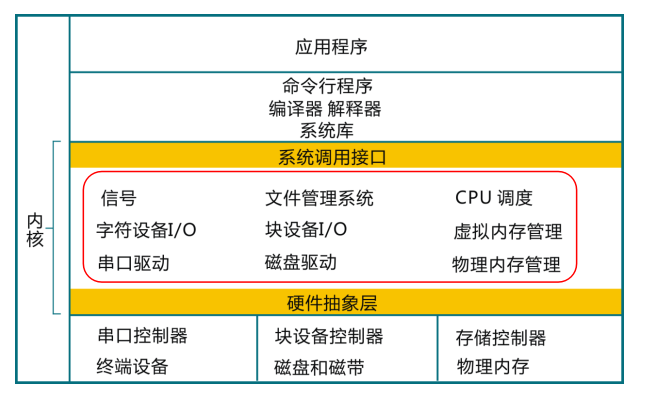
\includegraphics[width=1\linewidth]{ucore-arch}
%			
%		\end{column}
%		
%	\end{columns}
	
\end{frame}

%------------------------------------------------
\begin{frame}
	\frametitle{教学内容}

	\begin{columns}

	\begin{column}{0.5\textwidth}
	
    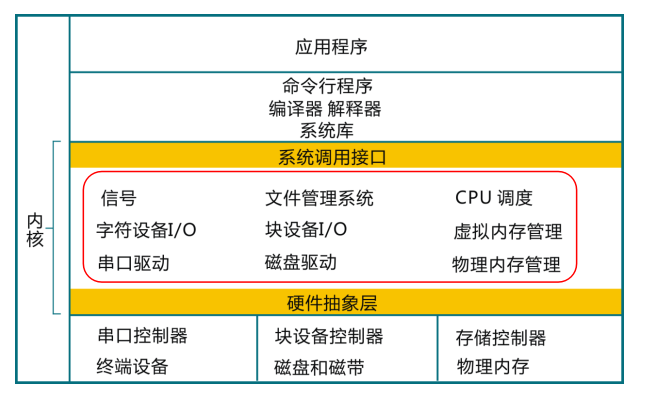
\includegraphics[width=1\linewidth]{ucore-arch}
    
    \end{column}
	
	\begin{column}{0.5\textwidth}
	\textbf{操作系统原理与实现}
    \begin{itemize}
		\item 操作系统结构
		\item 中断及系统调用 %\pause
		\item 内存管理
		\item 进程管理
		\item 处理机调度
		\item 同步互斥 %\pause
		\item 文件系统
		\item I/O子系统
    \end{itemize}
    
    \end{column}

\end{columns}

\end{frame}

%------------------------------------------------
\begin{frame}
	\frametitle{教学内容}

	\begin{columns}
    \begin{column}{0.6\textwidth}
        \begin{itemize}
            \item 操作系统概述
            \item 中断、异常与系统调用
            \item 进程与调度
            \item 存储管理
            \item 物理内存管理
            \item 虚拟存储概念
            \item 虚拟存储:局部页面置换算法
            \item 虚拟存储:全局页替换算法
            \item 进程、线程和协程
            \item 进程和线程控制
            \item 处理机调度
            \item 多处理器调度
        \end{itemize}
    \end{column}
	
	\begin{column}{0.4\textwidth}
    \begin{itemize}
        \item 同步互斥
        \item 信号量与管程
        \item 死锁和并发错误检测
        \item 进程通信
        \item 文件系统
        \item 文件系统实例
        \item I/O子系统
        \item 分布式系统
        \item 异步操作系统
        \item 操作系统虚拟化
        \item 操作系统的发展趋势
    \end{itemize}
    
    \end{column}

\end{columns}

\end{frame}

%------------------------------------------------
    \begin{frame}
        \frametitle{作业与实验}
        \begin{itemize}
            \item 平时作业
        \begin{itemize}
    		\item 课上练习与交流
	    	\item 课后练习
        \end{itemize} %\pause

            \item 基础实验
    \begin{itemize}
		\item r/u Core实验:面向RISC-V CPU用Rust/C写操作系统
    \end{itemize}
            \item 课程设计(大实验)
        \end{itemize}
\end{frame}

%------------------------------------------------
\begin{frame}
\frametitle{基础实验:面向RISC-V CPU用Rust/C写操作系统}
\begin{columns}
	
\begin{column}{0.4\textwidth}
\begin{itemize}
        \item 实验一:中断与任务切换
        \begin{itemize}
                \item ch0:操作系统实验准备
                \item ch1:程序与执行环境
                \item ch2:批处理系统
                \item ch3:多道与分时
        \end{itemize}

        \item 实验二(ch4):地址空间
\end{itemize}

\end{column}
 
\begin{column}{0.6\textwidth}
    \begin{itemize}
                \item 实验三(ch5):进程及进程管理
                \item 实验四(ch6):进程间通信
                \item 实验五(ch7):文件系统与I/O重定向
                \item 实验六(ch8):内核测试和优化(选项)
        \end{itemize}
\end{column}

\end{columns}

\end{frame}



%------------------------------------------------
\begin{frame}
\frametitle{课程设计}
	\begin{itemize}
	\item 各种CPU平台上的操作系统移植
		\begin{itemize}	
		\item RISC-V、x86-64、x86-32、MIPS、ARM
		\end{itemize}
	\item 操作系统内核功能实现和扩展
		\begin{itemize}	
		\item GUI、驱动、内核可加载模块、微内核
		\end{itemize} \pause
	\item 操作系统分析工具	
		\begin{itemize}	
		\item 错误分析、行为分析、模拟器
		\end{itemize}
	\item 操作系统新方向探索
		\begin{itemize}	
		\item Rust、内核语言、异步操作系统
		\end{itemize} \pause
	\item 参与操作系统相关比赛

		\begin{itemize}	
		\item \href{https://github.com/oscomp/os-competition-info}{全国全国大学生操作系统设计比赛}
		\item \href{https://www.opengcc.org/article/63/270.html}{中国软件开源创新大赛}
        \item \href{https://summer.iscas.ac.cn/#/org/projectlist}{开源软件供应链点亮计划}
		\end{itemize}
	\end{itemize}
\end{frame}
%------------------------------------------------
    
\begin{frame}[fragile]
    \frametitle{成绩评定}
    \begin{itemize}
        %\item 作业:5分
        \item 实验:30分
        \begin{itemize}
            \item 独立完成操作系统实验,并提交实验报告
        \end{itemize} %\pause
        \item 考试或课程设计:70分
        \begin{itemize}
            \item 期中考试:30分
            \item 期末考试:40分
            \item 有余力和兴趣的同学,可用课程设计替代考试
        \end{itemize}

    \end{itemize} %\pause

    总成绩加权方法:上述各项成绩的总和会做一次调整,基本原则是,各分数段保持一定的比例,可能的参考比例为A+/A/A-占25\%、B+/B/B-占45\%、C+/C/C-占20\%和D+/D/F占10\%。 

\end{frame}

%------------------------------------------------
    
    \begin{frame}
        \frametitle{作业:调查问卷}
        \begin{itemize}
            \item 为什么要学这门课? %\pause
            \item 你打算如何来学这门课?
            \item 对自己的课程学习要求是什么?
            \item 你愿意如实报告是否独立完成实验任务?
            \item 你希望在操作系统课上学到什么知识和什么能力? %\pause
            \item 以前的学习情况?
            \item 对计算机专业的看法是什么? %\pause
            \item 采集仅限于清华和学堂在线的操作系统课内注册的同学信息
        \end{itemize}
        
    \newline
    \newline
    
    注:作为认真思考后选课的依据,要求所有选课同学在课后一天内完成问卷填写。
    
    详见:\href{http://oscourse2019.mikecrm.com/te8s1h2}{2021年春季学期操作系统课选课问卷} ( 访问密码:Ngm25L )
    
    \end{frame}
%----------------------------------------------------------------------------------------

\end{document}
